\section{Data Preprocessing and Proxy-State Construction}

\subsection{Why Preprocessing Must Be Part of the Theory}

For the present project, data preprocessing is not a secondary engineering detail.
It determines whether the downstream learning problem can be interpreted as a causal state-transition identification problem.

If one trains directly on raw asynchronous sensor streams, the network must jointly solve:
\begin{itemize}
  \item multi-rate temporal alignment,
  \item denoising and bias suppression,
  \item sparse-observation completion,
  \item and controlled dynamics learning.
\end{itemize}

This coupling makes the optimization target ill-posed for short-horizon rollout.
Therefore, the preprocessing pipeline must be described explicitly in the mathematical method section.

\subsection{Raw Sensor Streams}

The raw data sources are:
\begin{itemize}
  \item PWM commands at $100\,\mathrm{Hz}$,
  \item IMU measurements at $100\,\mathrm{Hz}$,
  \item DVL velocity observations at approximately $10\,\mathrm{Hz}$,
  \item motor power observations at approximately $5\,\mathrm{Hz}$.
\end{itemize}

These signals do not arrive on a common time axis and do not play the same role in the transition problem.
Representative raw measurements are shown in Fig.~\ref{fig:raw-sensors}.

\begin{figure}[htbp]
  \centering
  \begin{subfigure}[t]{0.49\textwidth}
    \centering
    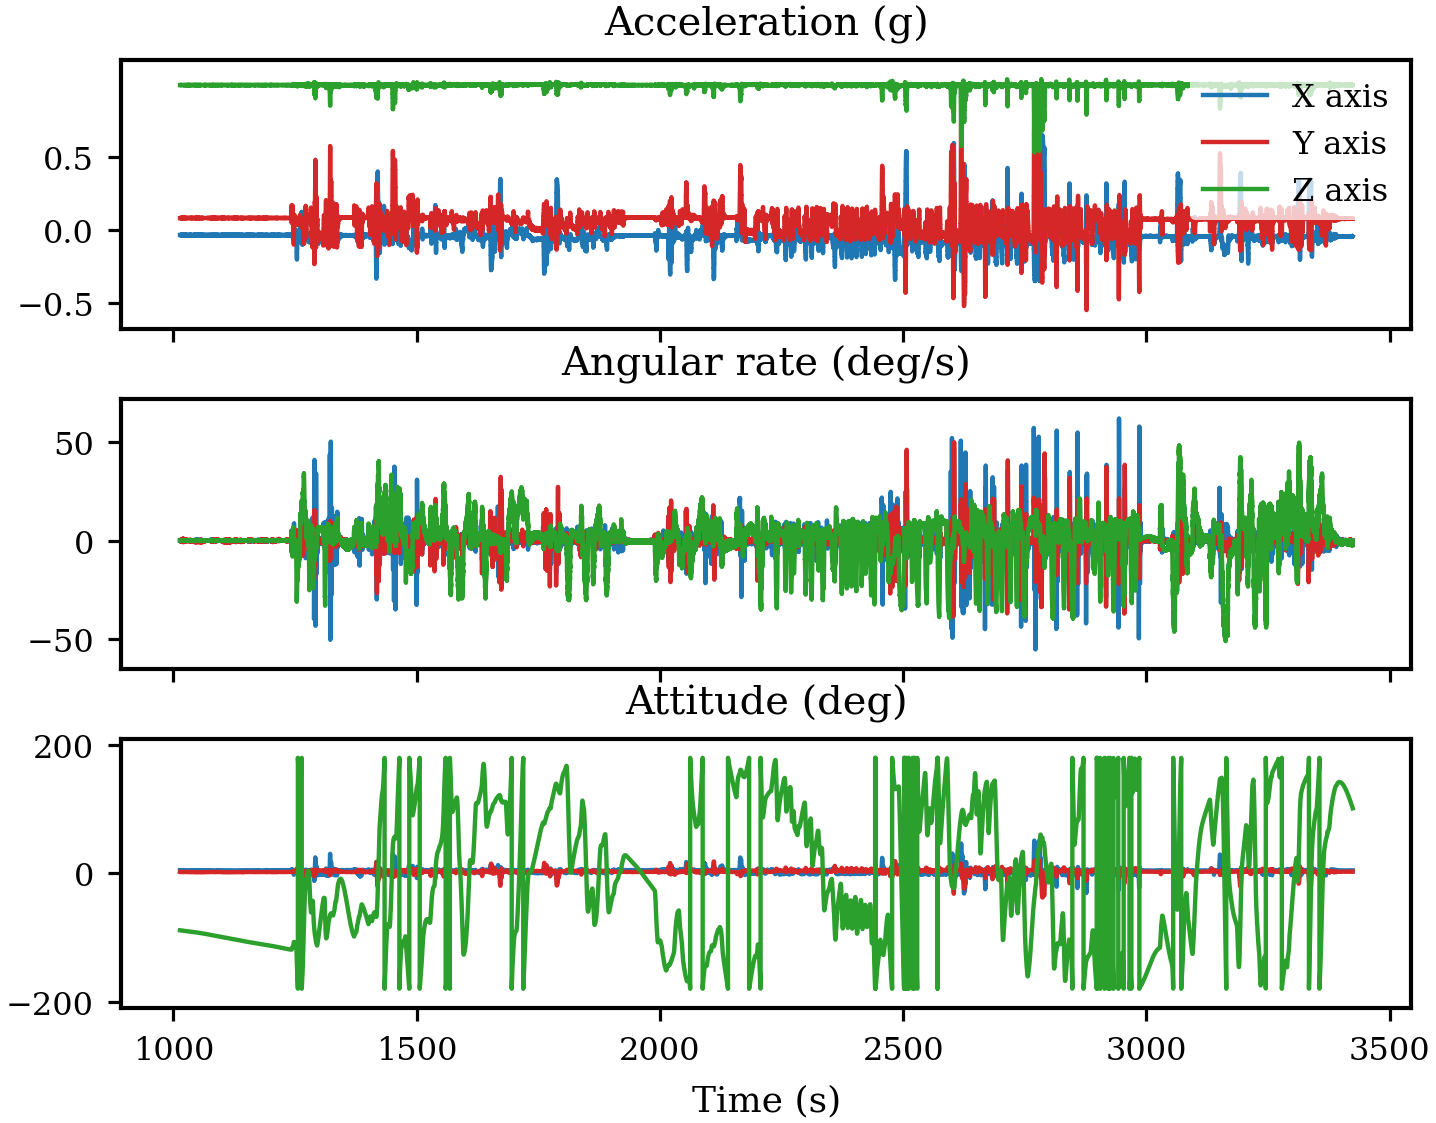
\includegraphics[width=\linewidth]{figures/pooltest02_imu_raw_9axis.png}
    \caption{Raw IMU example.}
  \end{subfigure}
  \hfill
  \begin{subfigure}[t]{0.49\textwidth}
    \centering
    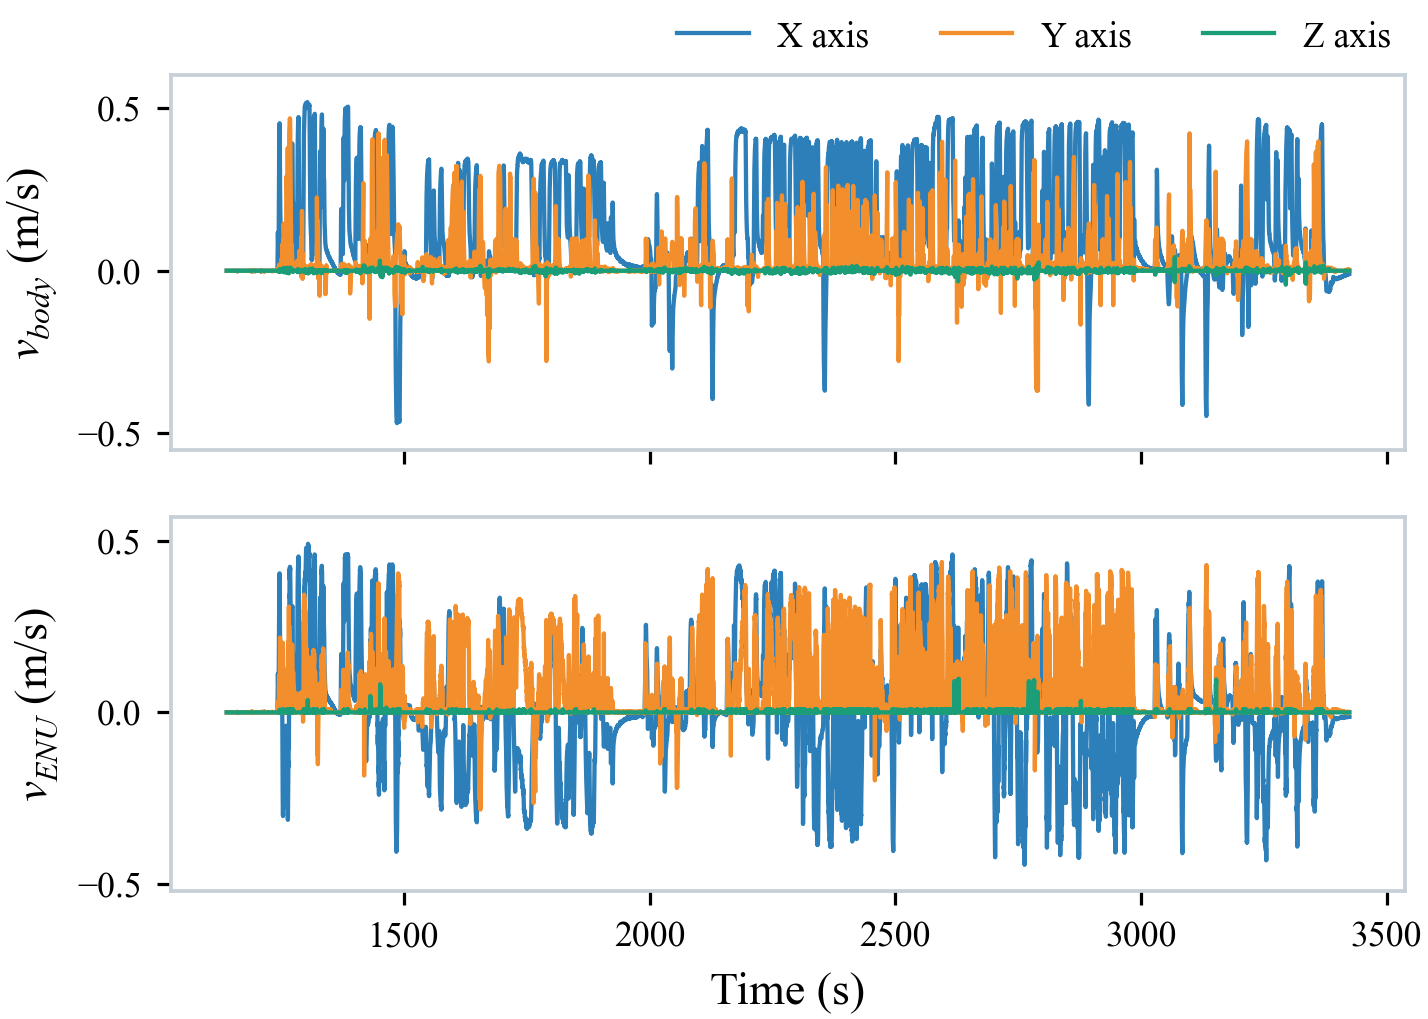
\includegraphics[width=\linewidth]{figures/pooltest02_dvl_raw_bi_be.png}
    \caption{Raw DVL example.}
  \end{subfigure}
  \caption{Representative raw sensor observations from the pool test dataset. The IMU provides dense body-motion evidence, while the DVL supplies lower-rate velocity observations.}
  \label{fig:raw-sensors}
\end{figure}

\subsection{IMU Preprocessing}

Let the accelerometer and gyroscope observations be denoted by
\begin{align}
\tilde{\mathbf{a}}_k &= \mathbf{a}_k - \mathbf{R}_{bn,k}\mathbf{g} + \mathbf{b}_{a,k} + \mathbf{n}_{a,k}, \\
\tilde{\boldsymbol{\omega}}_k &= \boldsymbol{\omega}_k + \mathbf{b}_{\omega,k} + \mathbf{n}_{\omega,k},
\end{align}
where $\mathbf{R}_{bn,k}$ is the body-to-navigation rotation, $\mathbf{g}$ is gravity, $\mathbf{b}_{a,k}$ and $\mathbf{b}_{\omega,k}$ are sensor biases, and $\mathbf{n}_{a,k}, \mathbf{n}_{\omega,k}$ denote measurement noise.

The IMU preprocessing chain applies:
\begin{enumerate}
  \item frame transformation into the training body frame,
  \item gravity compensation,
  \item bias correction,
  \item and light filtering for numerical stability.
\end{enumerate}

The purpose is not to create a perfect inertial solution, but to provide a cleaner high-rate propagation signal for the subsequent causal fusion stage.
An example of the processed IMU output is shown in Fig.~\ref{fig:imu-proc}.

\begin{figure}[htbp]
  \centering
  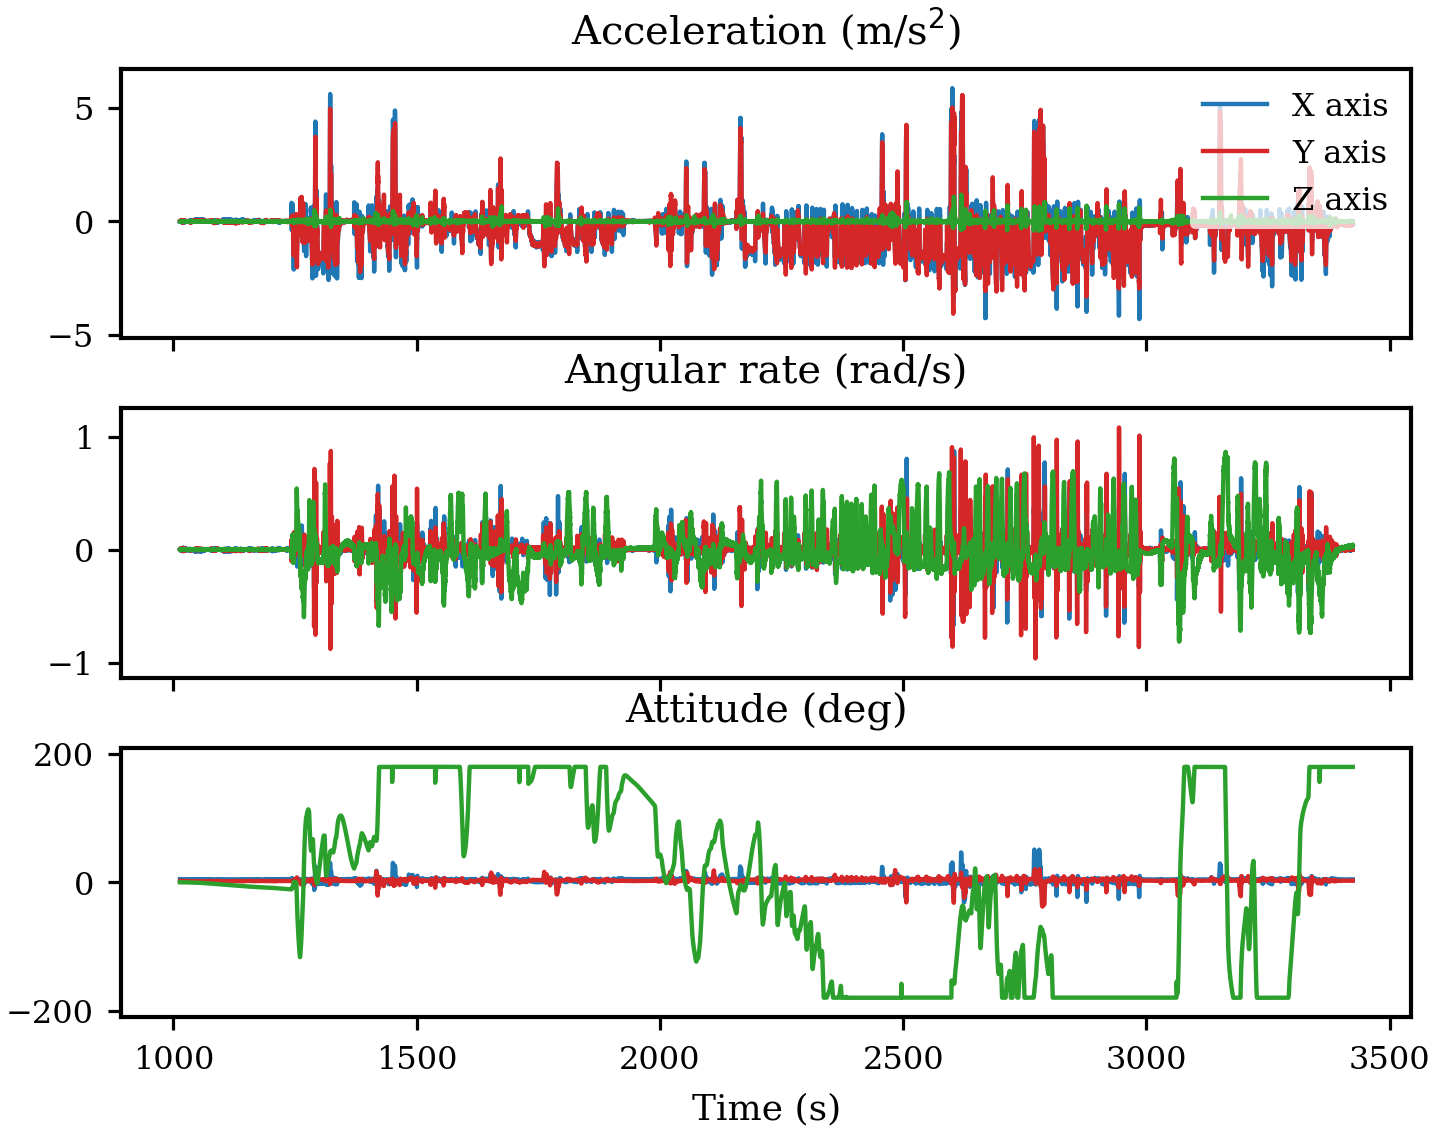
\includegraphics[width=0.64\textwidth]{figures/pooltest02_imu_proc_3rows.png}
  \caption{Example of the IMU preprocessing output after frame conversion, gravity handling, bias correction, and filtering.}
  \label{fig:imu-proc}
\end{figure}

\subsection{Multi-Rate Alignment}

All observations are projected onto a common master axis with sampling interval $\Delta t = 0.01\,\mathrm{s}$.
This aligned axis serves two purposes:
\begin{itemize}
  \item it makes the control input and state proxy share the same temporal semantics;
  \item it converts the learning problem into a discrete-time transition problem indexed by $k$.
\end{itemize}

The aligned training table therefore acts as the bridge between raw logging and transition-model learning.

\subsection{Causal KF / ESKF Fusion}

After alignment, a causal KF / ESKF stage combines high-rate IMU propagation with sparse DVL corrections.
The propagation step can be written abstractly as
\begin{align}
\hat{\mathbf{s}}_{k|k-1} &= f_{\mathrm{imu}}\!\left(\hat{\mathbf{s}}_{k-1|k-1}, \tilde{\mathbf{a}}_k, \tilde{\boldsymbol{\omega}}_k\right), \\
\mathbf{P}_{k|k-1} &= \mathbf{F}_k \mathbf{P}_{k-1|k-1}\mathbf{F}_k^{\top} + \mathbf{Q}_k,
\end{align}
where $\hat{\mathbf{s}}_{k|k-1}$ denotes the predicted internal state and $\mathbf{P}_{k|k-1}$ its covariance.

When a valid DVL measurement is available, the velocity-related update is applied:
\begin{align}
\mathbf{z}^{v}_k &= \mathbf{H}_k \hat{\mathbf{s}}_{k|k-1} + \mathbf{r}_k, \\
\mathbf{K}_k &= \mathbf{P}_{k|k-1}\mathbf{H}_k^{\top}
\left(
\mathbf{H}_k \mathbf{P}_{k|k-1}\mathbf{H}_k^{\top} + \mathbf{R}_k
\right)^{-1}, \\
\hat{\mathbf{s}}_{k|k} &= \hat{\mathbf{s}}_{k|k-1} +
\mathbf{K}_k\left(\mathbf{z}^{v}_k - \mathbf{H}_k \hat{\mathbf{s}}_{k|k-1}\right).
\end{align}

The output of this stage is not a full navigation solution for external deployment.
Instead, it is a causally estimated training-oriented proxy state:
\begin{equation}
\hat{\mathbf{x}}_k =
\begin{bmatrix}
\hat{\mathbf{a}}_k \\
\hat{\boldsymbol{\omega}}_k \\
\hat{\mathbf{v}}_k
\end{bmatrix},
\end{equation}
together with attitude context and reliability-related quantities such as DVL freshness and velocity covariance proxies.

\subsection{From Raw Observations to Dense Proxy States}

The effect of the fusion stage is illustrated in Fig.~\ref{fig:kf-proxy}.
The dense IMU stream supplies propagation information, while the sparse DVL observations intermittently correct the velocity estimate.
The result is a dense proxy-state sequence that remains compatible with online rollout semantics.

\begin{figure}[htbp]
  \centering
  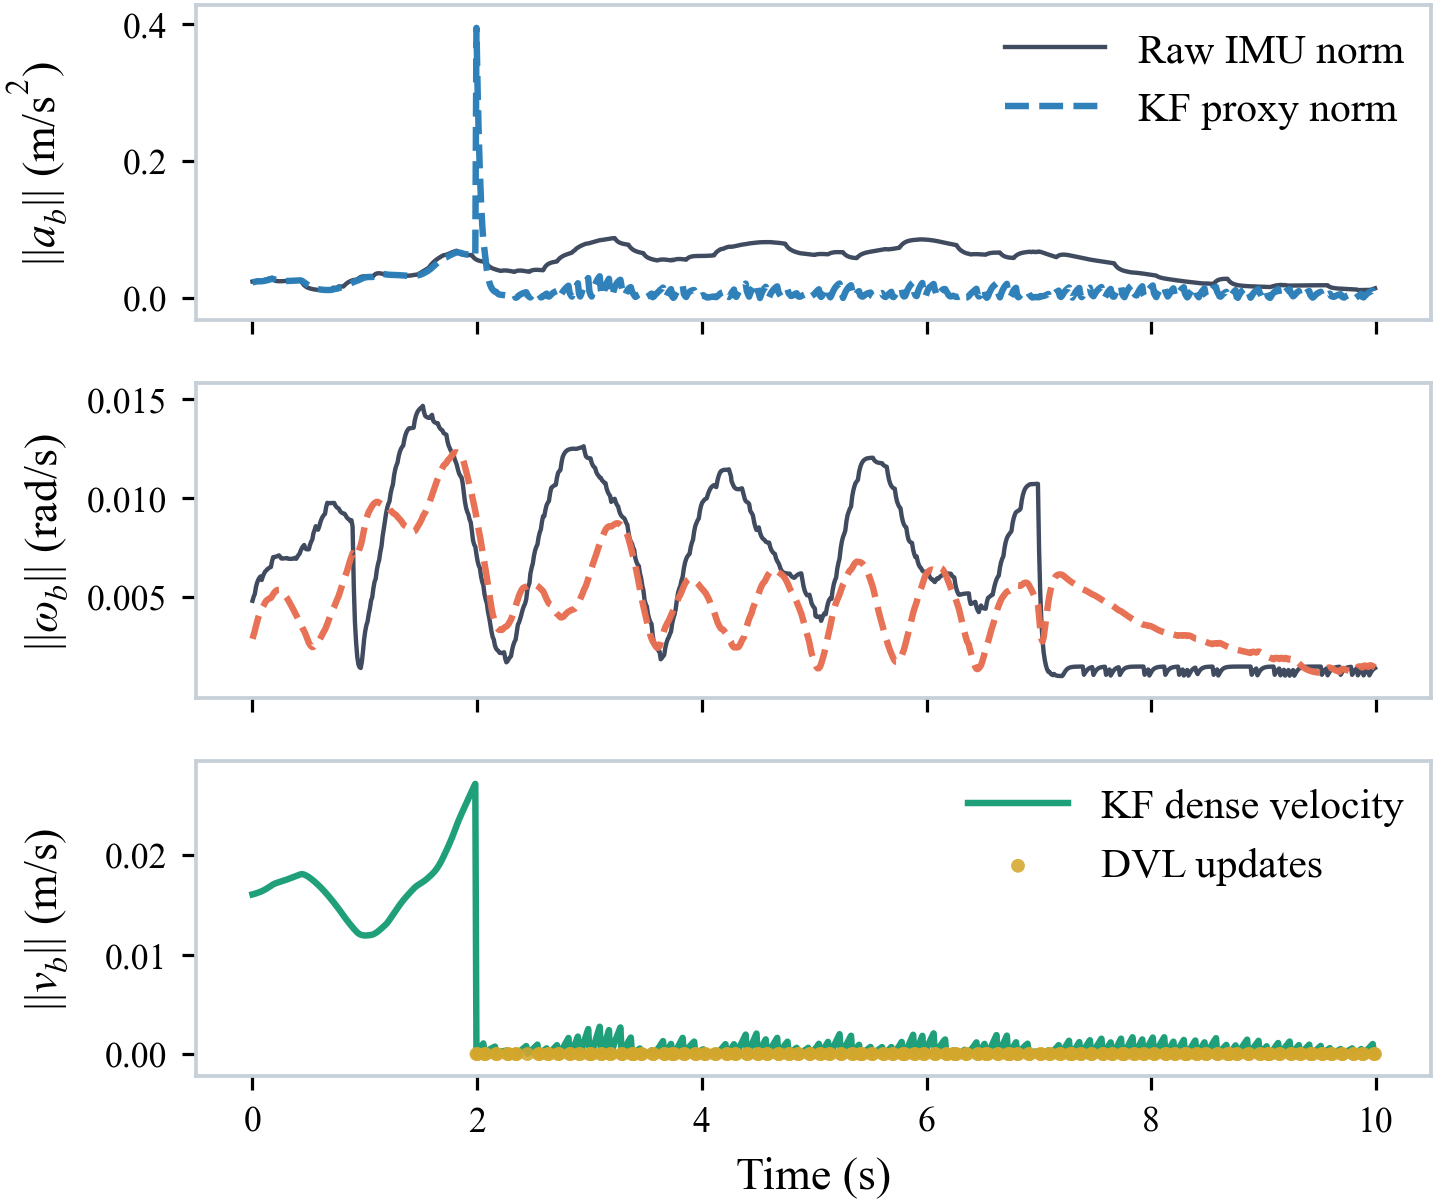
\includegraphics[width=0.66\textwidth]{figures/pooltest02_kf_proxy_overview.png}
  \caption{Example of proxy-state construction on the aligned training base table. The KF proxy suppresses raw IMU noise and turns sparse DVL velocity updates into a dense rollout-compatible velocity state.}
  \label{fig:kf-proxy}
\end{figure}

\subsection{Full-Run Visual Audit}

Short windows are useful for local interpretation, but they are insufficient for judging whether preprocessing quality is stable over an entire experiment.
For this reason, the current documentation also keeps a full-run visual audit, shown in Fig.~\ref{fig:kf-fullrun}.

This full-run figure serves three purposes:
\begin{itemize}
  \item it checks whether the KF proxy remains bounded over the whole trajectory,
  \item it reveals whether DVL corrections are frequent enough to suppress inertial drift,
  \item it helps identify non-physical spikes, rejected measurements, and long segments with stale velocity correction.
\end{itemize}

\begin{figure}[htbp]
  \centering
  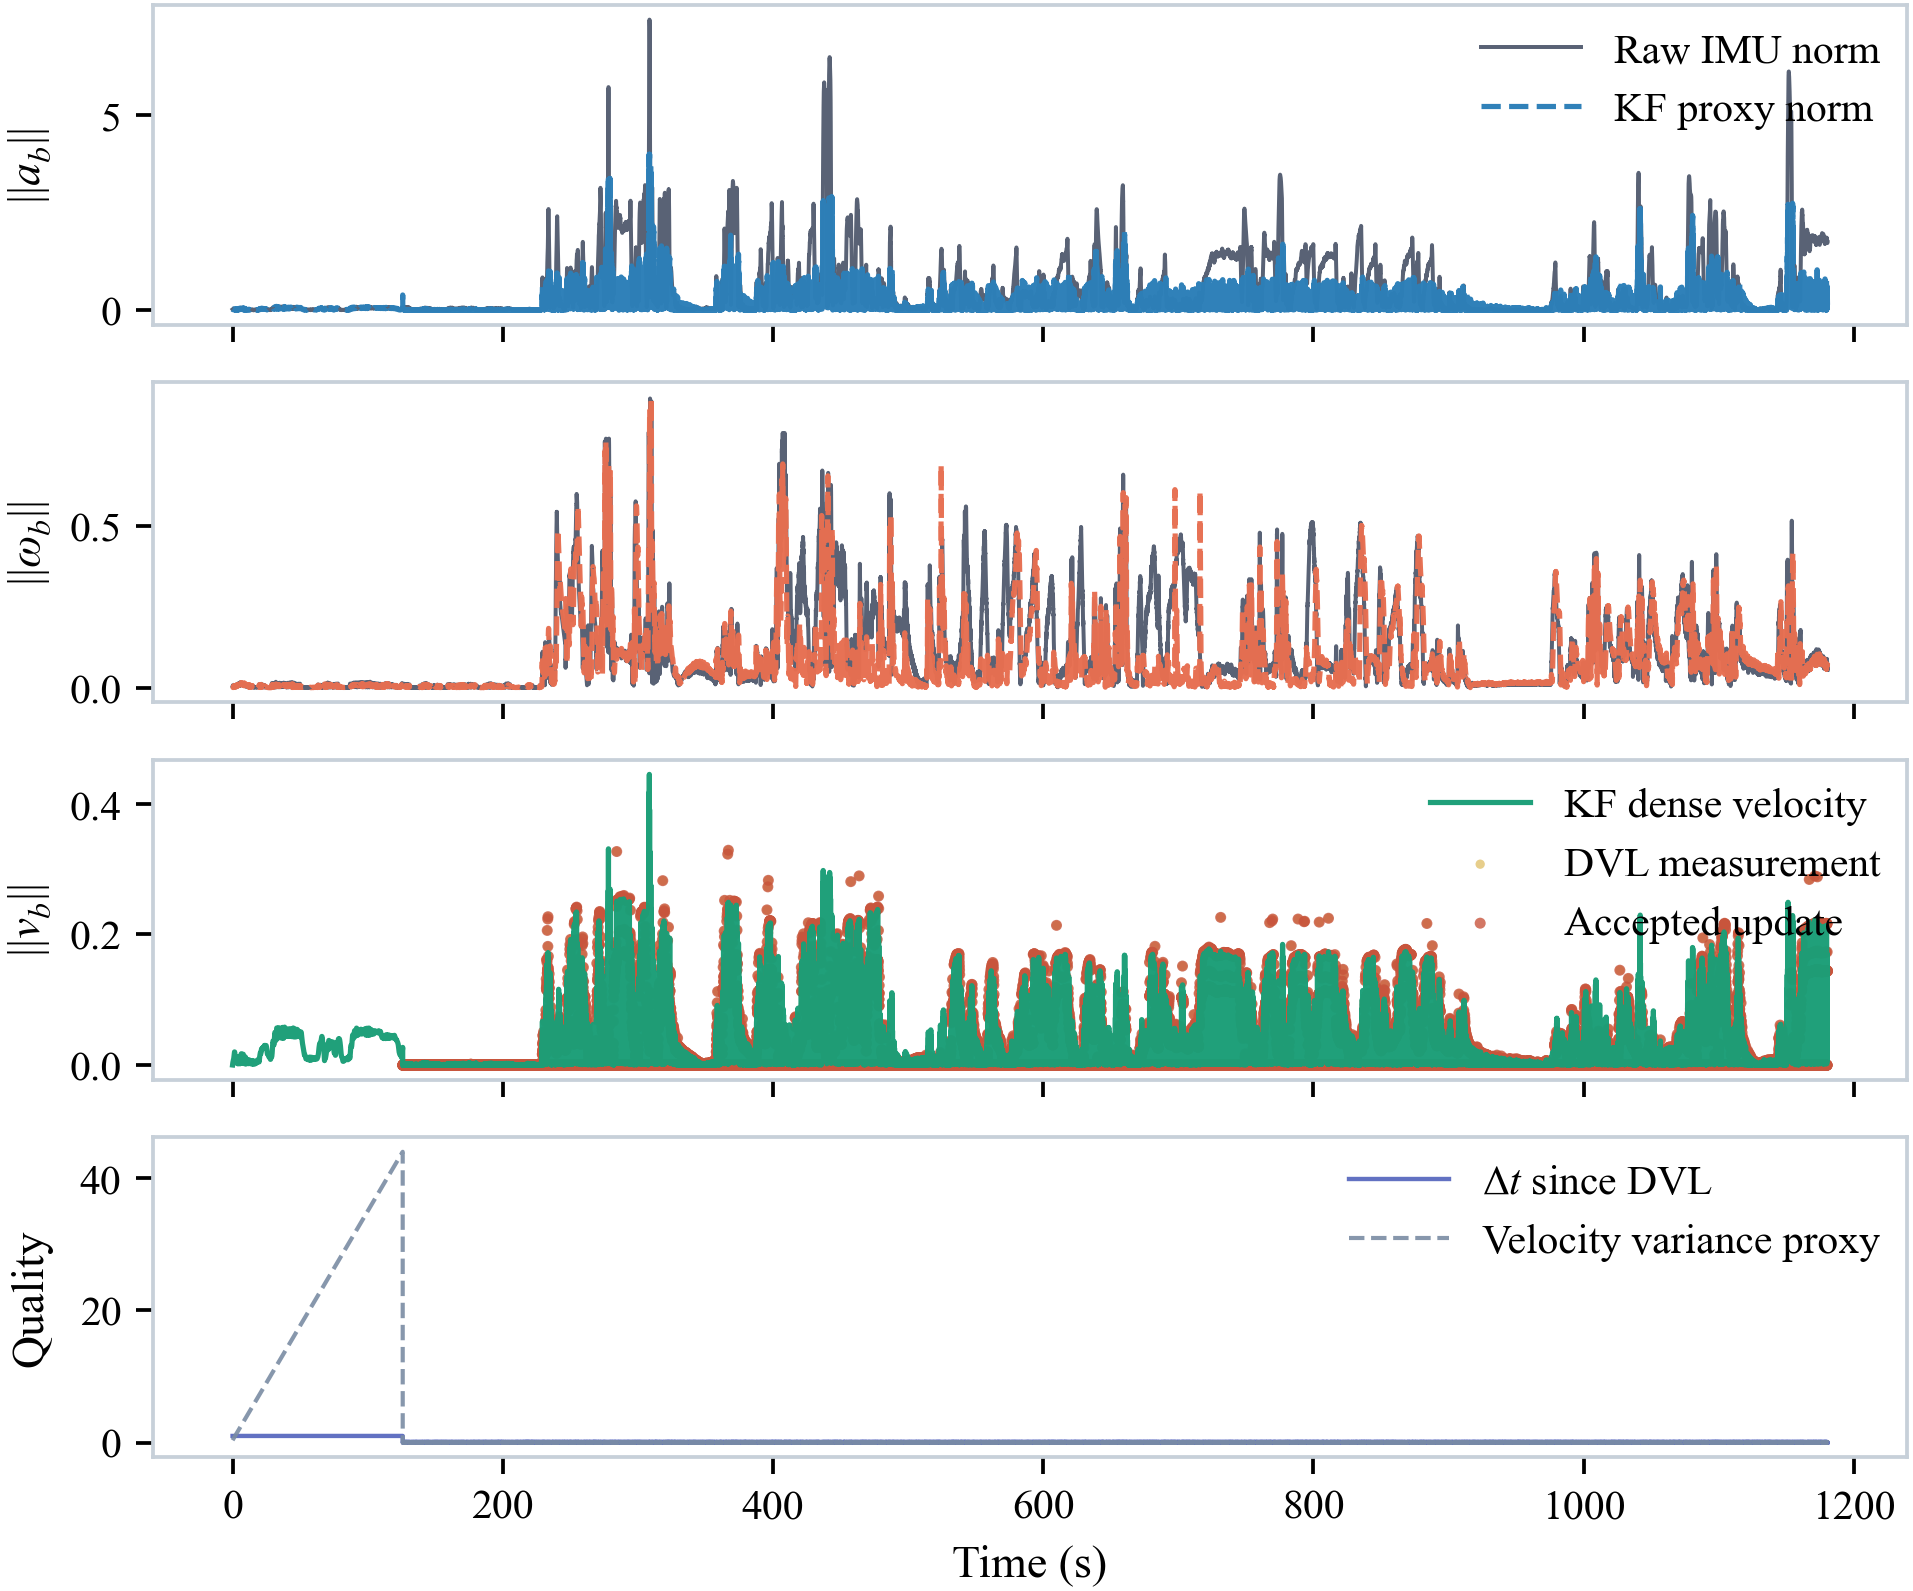
\includegraphics[width=0.84\textwidth]{figures/pooltest02_kf_proxy_fullrun.png}
  \caption{Full-run visual audit of the preprocessing and fusion output. This figure is intended for method validation rather than presentation-only illustration, because it exposes drift, correction freshness, variance growth, and possible outlier behavior over the complete experiment.}
  \label{fig:kf-fullrun}
\end{figure}

\subsection{Training Precursor Interpretation}

The preprocessing pipeline leads to the following modeling stance:
\begin{itemize}
  \item PWM is treated as the primary control input,
  \item $\hat{\mathbf{x}}_k$ is treated as the causal proxy state,
  \item attitude and quality fields are treated as context variables.
\end{itemize}

Hence, the network is not trained to recover state directly from raw heterogeneous observations.
Instead, it is trained on
\begin{equation}
\mathbf{z}_k =
\begin{bmatrix}
\mathbf{u}_k \\
\hat{\mathbf{x}}_k \\
\mathbf{c}_k
\end{bmatrix},
\end{equation}
which is mathematically much closer to a discrete-time controlled state-transition problem.

This preprocessing-aware viewpoint is the reason the current project can move from sequence fitting toward a solver-style model:
\begin{equation}
\hat{\mathbf{x}}_{k+1} = f_{\theta}\!\left(\hat{\mathbf{x}}_k, \mathbf{u}_k, \mathbf{c}_k\right).
\end{equation}
